\documentclass[tikz,border=2pt]{standalone}
\usepackage{amsmath}
\usepackage{pgfplots}
\pgfplotsset{compat=1.18}
\usetikzlibrary{arrows.meta}
\begin{document}
% Exponential losses with fitted rate 2/70, observed only above d = 100: the ground-up density f_theta (thin) has
% almost all its mass below d; dividing by bar F_theta(100) = e^{-20/7} gives the conditional density on x > 100,
% and the observations 120, 150 contribute f_theta(x_i)/bar F_theta(d).
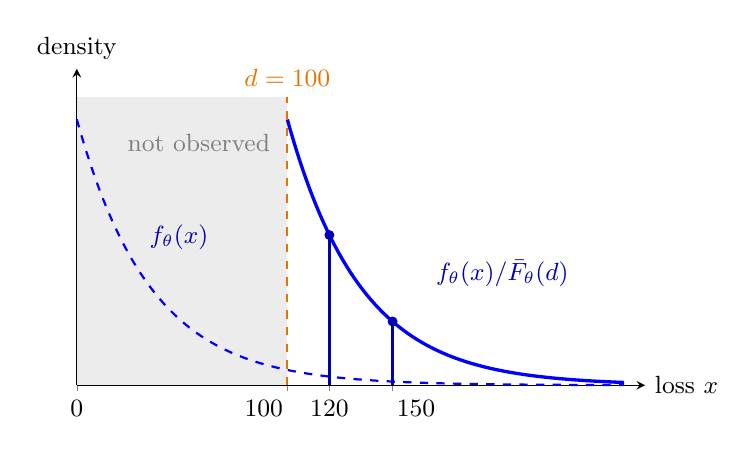
\begin{tikzpicture}[font=\small, >={Latex[length=2mm]}]
  \begin{axis}[
    axis lines=left, xmin=0, xmax=270, ymin=0, ymax=0.034,
    xtick={0,100,120,150}, xticklabels={$0$,\makebox[0pt][r]{$100$\,},$120$,\makebox[0pt][l]{\,$150$}}, ytick=\empty,
    xlabel={loss $x$}, ylabel={density},
    xlabel style={at={(axis description cs:1,0)}, anchor=west},
    ylabel style={rotate=-90, at={(axis description cs:0,1)}, anchor=south},
    samples=120, width=8.8cm, height=5.6cm, clip=false]
    \fill[gray!15] (axis cs:0,0) rectangle (axis cs:100,0.031);
    \node[gray, align=center] at (axis cs:58,0.026) {not observed};
    % ground-up density
    \addplot[blue, thick, dashed, domain=0:260] {(2/70)*exp(-2*x/70)};
    \node[blue!70!black, anchor=south west] at (axis cs:30,0.0135) {$f_\theta(x)$};
    % conditional (renormalised) density on x > d
    \addplot[blue, very thick, domain=100:260] {(2/70)*exp(-2*(x-100)/70)};
    \node[blue!70!black, anchor=west] at (axis cs:166,0.012) {$f_\theta(x)/\bar F_\theta(d)$};
    % observations
    \draw[blue!70!black, thick] (axis cs:120,0) -- (axis cs:120,0.016134);
    \draw[blue!70!black, thick] (axis cs:150,0) -- (axis cs:150,0.006848);
    \fill[blue!70!black] (axis cs:120,0.016134) circle (1.8pt);
    \fill[blue!70!black] (axis cs:150,0.006848) circle (1.8pt);
    % truncation point
    \draw[orange!90!black, thick, dashed] (axis cs:100,0) -- (axis cs:100,0.031);
    \node[orange!90!black, anchor=south] at (axis cs:100,0.031) {$d=100$};
  \end{axis}
\end{tikzpicture}
\end{document}
